%----------------------------------------------------------------------------------------
%	INFORMATIONS DOCUMENT ET PACKAGES
%----------------------------------------------------------------------------------------

\documentclass[12pt,a4paper]{article}
\usepackage[utf8]{inputenc}
\usepackage[T1]{fontenc}
\usepackage[french]{babel}
\usepackage{textcomp}
\usepackage{array,multirow,makecell}
\usepackage{lmodern}
\usepackage{geometry}
\usepackage{graphicx}
\usepackage{xcolor}
\usepackage{titlesec}
\usepackage{titletoc}
\usepackage{fancyhdr}
\usepackage{enumitem}
\usepackage{hyperref}

%----------------------------------------------------------------------------------------
%	PAGE D'ACCUEIL
%----------------------------------------------------------------------------------------

\hypersetup{pdfstartview=XYZ}
\frenchbsetup{StandardLists=true}
\geometry{hmargin=2.5cm,vmargin=2cm}
\pagestyle{empty}
\addto\captionsfrench{\renewcommand{\contentsname}{Sommaire}}
\begin{document}

    \begin{titlepage}
        \fontfamily{phv}\selectfont
        \vspace*{\stretch{1}}
        \begin{flushright}\LARGE
            Christoph Samuel
        \end{flushright}
        \hrule
        \begin{flushleft}\huge\bfseries
            La programmation informatique
        \end{flushleft}
        \vspace*{\stretch{2}}
        \begin{center}
            Avril 2021
        \end{center}
    \end{titlepage}
    
    \addto\captionsfrench{\renewcommand{\abstractname}{La programmation informatique}}
    \setcounter{tocdepth}{3}
    
%----------------------------------------------------------------------------------------
%	SOMMAIRE
%----------------------------------------------------------------------------------------
    
    \clearpage
    
    \tableofcontents
    \listoffigures
    \listoftables
    \vspace{2,5cm}
    
    \begin{abstract}
        Le document porte sur la programmation informatique, dans un premier temps nous verrons une bréve histoire sur la programmation\ref{histoire} ensuite nous verrons ses différentes pratiques\ref{pr}, pour enfin finir sur la création un programme informatique et les différents types de programmation\ref{3} dans l'informatique.
    \end{abstract}
    
%----------------------------------------------------------------------------------------
%	DEBUT DE LA PRESENTATION
%----------------------------------------------------------------------------------------
    
    \newpage
    
%----------------------------------------------------------------------------------------
    
    \section{Introduction}
    La programmation dans le domaine informatique est l'ensemble des activités qui permettent l'écriture des programmes informatiques. C'est une étape importante de la conception de logiciel (voire de matériel).Pour écrire le résultat de cette activité, on utilise un \textit{langage de programmation\footnote{notation conventionnelle destinée à formuler des algorithmes et produire des programmes informatiques qui les appliquent}.}\\
    
%----------------------------------------------------------------------------------------
    
    \begin{figure}[!h]
        \centering
        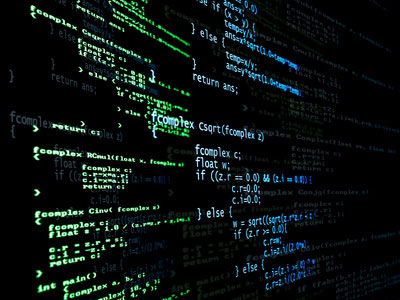
\includegraphics[height=100px, width=160px]{intro}
        \caption{Programmation informatique}
        \label{fig:introduction}
    \end{figure}
    
%----------------------------------------------------------------------------------------
    
    La programmation représente le plus souvent le codage, c’est-à-dire la rédaction du code source d'un logiciel. On utilise plutôt le terme développement pour lister l'ensemble des activités liées à la création d'un logiciel.
    
%----------------------------------------------------------------------------------------
    
    \section{\label{histoire}Une brève histoire de la programmation}
    La première machine programmable (c’est-à-dire machine dont les possibilités changent quand on modifie son "programme") est probablement le métier à tisser de Jacquard, qui a été réalisé en 1801. La machine utilisait une suite de cartons perforés. Les trous indiquaient le motif que le métier suivait pour réaliser un tissage.\\
    
%----------------------------------------------------------------------------------------
    
    \begin{figure}[!h]
        \centering
        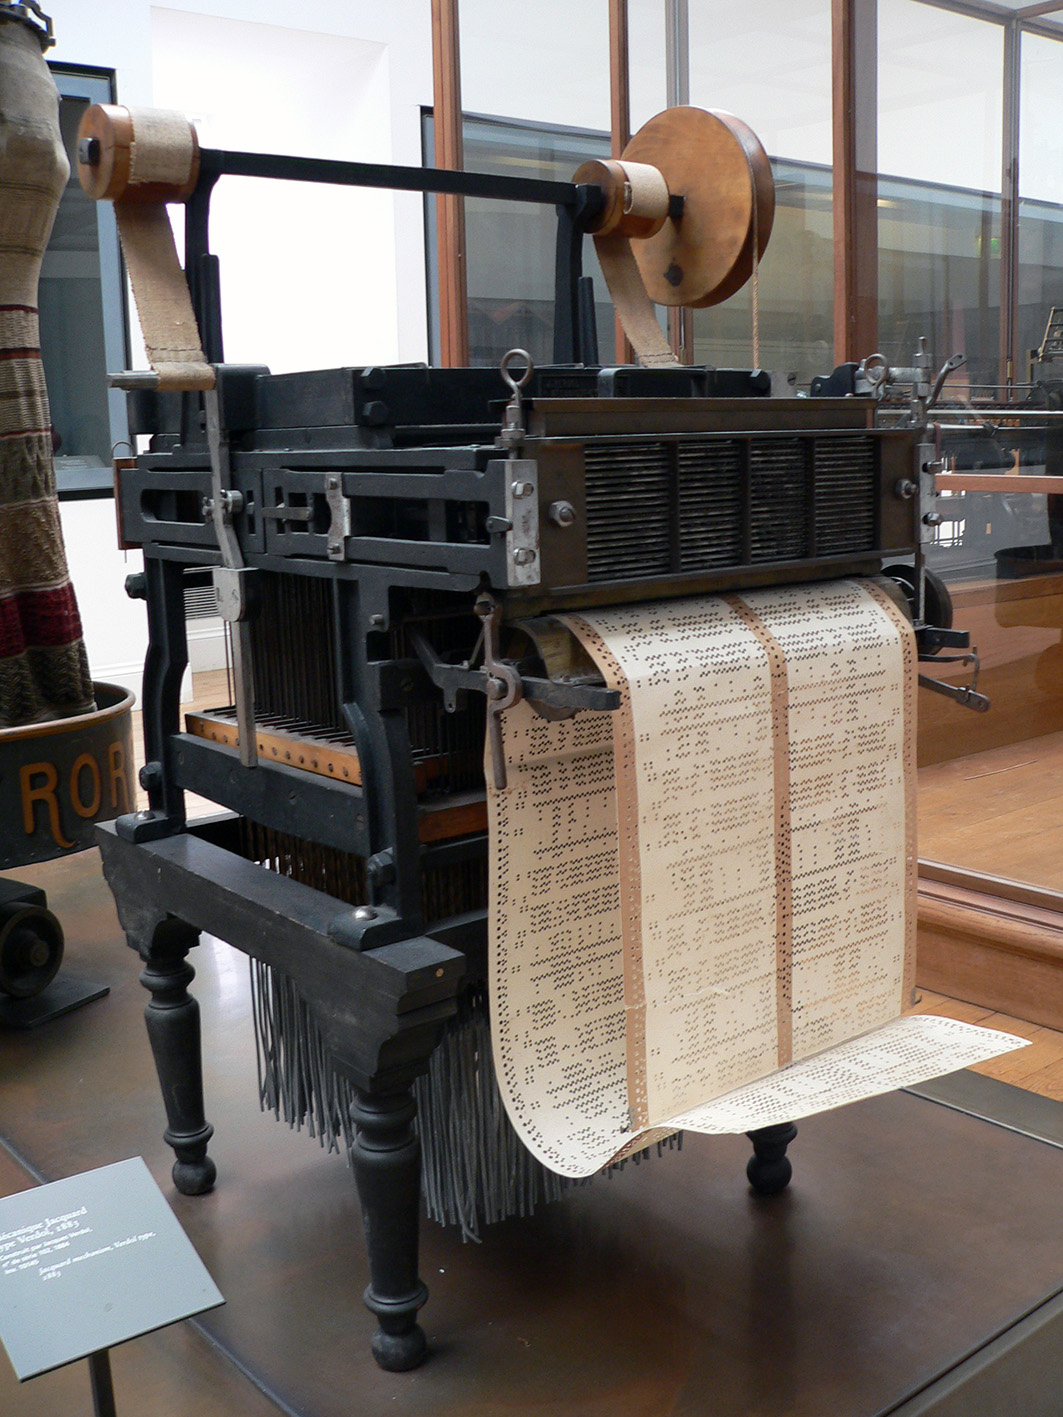
\includegraphics[height=215px, width=140px]{machine.jpg}
        \caption{Machine métier a tisser}
        \label{fig:Métier a tisser}
    \end{figure}
    
%----------------------------------------------------------------------------------------
    
    \newpage
    
%----------------------------------------------------------------------------------------
    
    Cette innovation a été ensuite améliorée par Herman Hollerith d'IBM pour le développement de la fameuse carte perforée d'IBM.\\
    
%----------------------------------------------------------------------------------------
    
    \begin{figure}[ht]
        \centering
        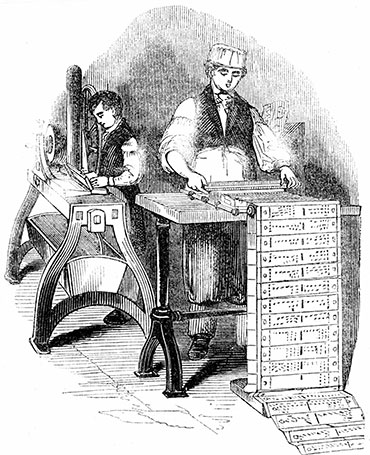
\includegraphics[height=160px, width=120px]{dessin.jpg}
        \caption{Métier a tisser version dessin}
        \label{fig:Métier a tisser version dessin}
    \end{figure}
    
%----------------------------------------------------------------------------------------
    
    En 1936, la publication de On Computable Numbers with an Application to the Entscheidungsproblem\cite{livre2}\footnote{article fondateur de la  science informatique} par Alan Mathison Turing donne le coup  d'envoi à la  création de l'ordinateur programmable. Il y présente sa machine de  Turing, le premier calculateur universel programmable, et invente les concepts et les termes de programmation et de programme. Les programmes devenant plus complexes, cela est devenu presque  impossible, parce qu'une seule erreur rendait le programme entier  inutilisable. Avec les progrès des supports de données, il devient possible de charger le programme à partir de cartes perforées, contenant la liste des instructions en code binaire spécifique à un type d'ordinateur particulier. La puissance des ordinateurs augmentant, on les utilisa pour faire les programmes, les programmeurs préférant naturellement rédiger du texte plutôt que des suites de 0 et de 1, à charge pour l'ordinateur d'en faire la traduction lui-même. Avec le temps, de nouveaux langages de programmation sont apparus, faisant de plus en plus abstraction du matériel sur lequel devaient tourner les programmes. Ceci plusieurs facteurs de gains : ces langages sont plus faciles à apprendre, un programmeur peut produire du code plus rapidement, et les programmes produits peuvent tourner sur différents types de machines.
    
%----------------------------------------------------------------------------------------
    
    \subsection{La fin des programmeurs ?}
    De tous temps, on a prédit « la fin des programmeurs ». Dans les années 60, les langages symboliques comme AUTO-CODE, Cobol et Fortran ont  en effet mis fin "en grande partie" à la programmation de bas niveau tel que l'assembleur\footnote{langage de plus bas niveau qui représente le langage machine sous une forme lisible par un humain.}. Il semblait alors clair que n'importe qui était capable d'écrire du code du type:

%----------------------------------------------------------------------------------------
    
    \begin{center}
        \begin{figure}[ht]
            \centering
             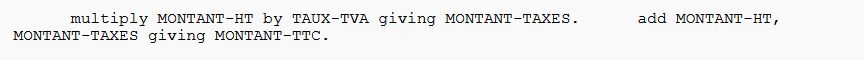
\includegraphics[height=40px, width=450px]{exemple1}
        \end{figure}
        
      ou
      
%----------------------------------------------------------------------------------------
    
    \newpage
    
%----------------------------------------------------------------------------------------
    
        \begin{figure}[ht]
            \centering
            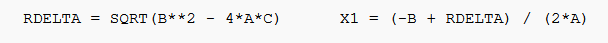
\includegraphics[height=25px, width=400px]{exemple2}
        \end{figure}  
        
        plutôt que des dizaines de lignes comme\\
        
        \begin{figure}[ht]
            \centering
            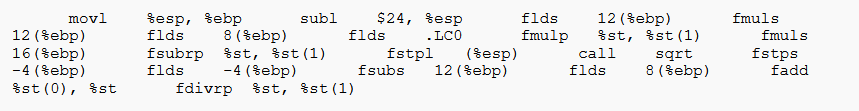
\includegraphics[height=60px, width=450px]{exemple3}
        \end{figure}
    \end{center}
    
%----------------------------------------------------------------------------------------
    
    Pourtant il a vite fallu se rendre compte que la programmation ne se limitait pas au codage, et que la conception d'applications était un vrai métier qui ne s'improvise pas.\\
   
%----------------------------------------------------------------------------------------
    
    \section{\label{pr}Pratique}
    En programmation informatique la pratique est établie sos plusieurs points parmis lesquel on retrouve l'algorithmique, la gestion de versions, l'optimisation du code, la programmation système, le refactoring et des tests (intégration et unitaire).
    
%----------------------------------------------------------------------------------------
    
    \begin{enumerate}[leftmargin=30px]
        \item L'algorithmique est l'étude et la production de règles et techniques impliquées dans la définition et la conception d'algorithmes.
        \item La gestion de versions consiste à gérer l'ensemble des versions d'un ou plusieurs fichiers, elle concerne surtout la gestion des codes source. 
        \item L'optimisation de code consiste à améliorer l'efficacité du code informatique d'un programme (plus rapide, moins de place mémoire...)
        \item La programmation système est un type de programmation qui vise au développement de programmes qui font partie du système d’exploitation d’un ordinateur ou qui en réalisent les fonctions.
        \item Le refactoring \footnote{réusinage de code} est l'opération consistant à retravailler le code source d'un programme informatique sans y ajouter des fonctionnalités de façon à en améliorer la lisibilité.
        \item Le test d'intégration est une phase de tests,vérifiant le bon fonctionnement d'une partie précise d'un logiciel.
    \end{enumerate}
    
%----------------------------------------------------------------------------------------
    
    \section{Phases de création d'un programme}
    On retrouve dans la programmation informatique une étape crutiale qui est la création d'un programme. Cette création s'effectue en 4 phases, une phase de conception suivie d'une phase de codage puis une phase de transforation du code source et pour finir le test du programme final.
    
%----------------------------------------------------------------------------------------
    
    \newpage
    
%----------------------------------------------------------------------------------------
    
    \subsection{Conception}
    La phase de conception définit le but du programme. Si on fait une rapide analyse fonctionnelle d'un programme, on détermine essentiellement les données qu'il va traiter (données d'entrée), la méthode employée (l'algorithme), et le résultat (données de sortie). Les données d'entrée et de sortie peuvent être de nature très diverses. On retrouve en général les mêmes fonctionnalités de base :\\
    
%----------------------------------------------------------------------------------------
    
    \textbf{\underline{Pour la programmation impérative}}\\
    
    \begin{enumerate}
        \item Si alors ( SI prédicat ALORS faire ceci SINON faire cela ),
        \item Tant que ( TANT QUE prédicat faire...),
        \item Pour ( Pour variable allant de borne inférieur à borne supérieur faire ...),
    \end{enumerate}

    \bigskip
    
%----------------------------------------------------------------------------------------
    
    \subsection{Codage}
    Une fois l'algorithme défini, l'étape suivante est de coder le programme. Le codage dépend de l'architecture sur laquelle va s'exécuter le programme, de compromis temps-mémoire, et d'autres contraintes. Ces contraintes vont déterminer quel langage de programmation utiliser pour "convertir" l'algorithme en code source.\\
    
%----------------------------------------------------------------------------------------
    
    \begin{figure}[ht]
        \centering
        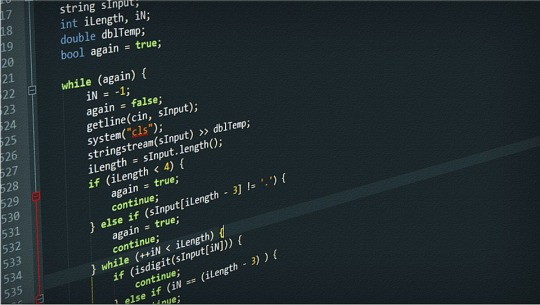
\includegraphics[height=60px, width=130px]{codage.jpg}
        \caption{Le codage}
        \label{fig:Le codage}
    \end{figure}
    
%----------------------------------------------------------------------------------------
    
    \subsection{Transformation du code source}
    Le code source\footnote{texte qui présente les instructions composant un programme sous une forme lisible} n'est (presque) jamais utilisable tel quel. Il est généralement écrit dans un langage "de haut niveau", compréhensible pour l'homme, mais pas pour la machine.\cite{article1}
    
%----------------------------------------------------------------------------------------
    
    \subsubsection{Compilation}
    Certains langages sont ce qu'on appelle des langages compilés\cite{article2}. En toute généralité, la compilation est l'opération qui consiste à transformer un langage source en un langage cible. Dans le cas d'un programme, le compilateur va transformer tout le texte représentant le code source du programme, en code compréhensible pour la machine, appelé code machine.Dans le cas de langages dits compilés, ce qui est exécuté est le résultat de la compilation. Une fois effectuée, l'exécutable obtenu peut être utilisé sans le code source.\\
    
%----------------------------------------------------------------------------------------
    
    \newpage
    
%----------------------------------------------------------------------------------------
    
    \begin{figure}[ht]
        \centering
        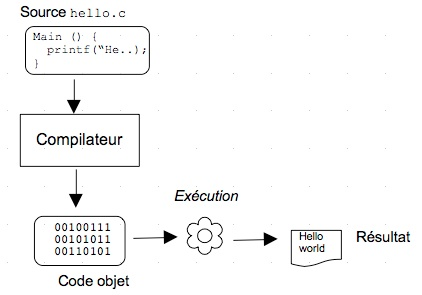
\includegraphics[height=180px, width=240px]{compilation.jpg}
        \caption{Exemple de compilation}
        \label{fig:Exemple de compilation}
    \end{figure}
    
%----------------------------------------------------------------------------------------
    
    Il faut également noter que le résultat de la compilation n'est pas forcément du code machine correspondant à la machine réelle, mais peut être du code compris par une machine virtuelle (c'est-à-dire un programme simulant une machine), auquel cas on parlera de bytecode\footnote{code intermédiaire entre les instructions machines et le code source, qui n'est pas directement exécutable}. C'est par exemple le cas en Java\footnote{Java est un langage de programmation orienté objet}. L'avantage est que, de cette façon, un programme peut fonctionner sur n'importe quelle machine réelle, du moment que la machine virtuelle existe pour celle-ci.\\
    
%----------------------------------------------------------------------------------------
    
    \subsubsection{Interprétation}
    D'autres langages ne nécessitent pas de phase spéciale de compilation. La méthode employée pour exécuter le programme est alors différente. Le programme entier n'est jamais compilé. Chaque ligne de code est compilée « en temps réel » par un programme. On dit de ce programme qu'il interprète le code source. Par exemple, python ou perl sont des langages interprétés.\\
    
%----------------------------------------------------------------------------------------
    
    \begin{figure}[ht]
        \centering
        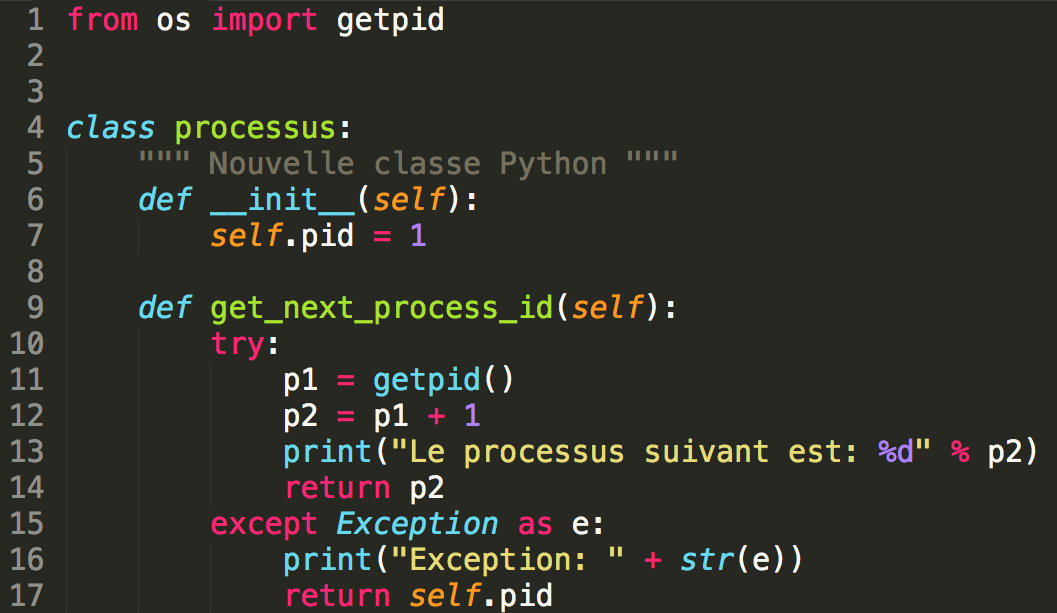
\includegraphics[height=150px, width=280px]{code_python.png}
        \caption{Un exemple de programmation en Python}
        \label{fig:Un exemple de programmation en Python}
    \end{figure}
    
%----------------------------------------------------------------------------------------
    
    \newpage
    
%----------------------------------------------------------------------------------------
    
    Cependant, ce serait faux de dire que la compilation n'intervient pas. 
    L'interprète produit le code machine, au fur et à mesure de l'exécution
    du programme, en compilant chaque ligne du code source.\\

%----------------------------------------------------------------------------------------

    \begin{table}
        \centering
        \begin{tabular}{ c  c  c  c  c } \\ 
            \hline
            langage de programmation & rang 2020 & rang 2015 & rang 2010 & rang 2005 \\
            \hline
            Java    & 1 & 2 & 1 & 2 \\ 
            \hline
            C       & 1 & 1 & 2 & 1 \\ 
            \hline
            Python  & 3 & 7 & 6 & 6 \\ 
            \hline
            C++     & 4 & 4 & 4 & 3 \\ 
            \hline
        \end{tabular}
        \caption{Classement des meilleurs languages de programmation depuis 2005}
        \label{2}
    \end{table}
    
%----------------------------------------------------------------------------------------

    \subsubsection{Avantages, inconvénients}
    Ces langages comportent tous des avantages, des inconvénients et leur domaines de pratique on retrouve donc des études et ouvrages pour chaqu'un d'eux par exemple avec The C programming language\cite{livre1} pour le C. Les avantages généralement retenus pour l'utilisation de langages "compilés", est qu'ils sont plus rapides à l'exécution que des langages interprétés, car l'interprète doit être lancé à chaque exécution du programme, ce qui mobilise systématiquement les ressources.\\ Traditionnellement, les langages interprétés offrent en revanche une certaine portabilité (la capacité à utiliser le code source sur différentes plates-formes), ainsi qu'une facilité pour l'écriture du code. En effet, il n'est pas nécessaire de passer par la phase de compilation pour tester le code source. Les quatres languages\ref{2} vu precédements sont les plus utilisés.
    
%----------------------------------------------------------------------------------------

    \subsection{Test du programme}
    C'est l'une des étapes les plus importantes de la création d'un programme. En principe, tout programmeur se doit de vérifier chaque partie d'un programme, de le tester. Il existe différents types de test. \\

%----------------------------------------------------------------------------------------

    \textbf{On peut citer en particulier :}
    \begin{enumerate}
        \item Test unitaire
        \item Test d'intégration
        \item Test de performance
    \end{enumerate}

%----------------------------------------------------------------------------------------

    \begin{figure}[ht]
        \centering
        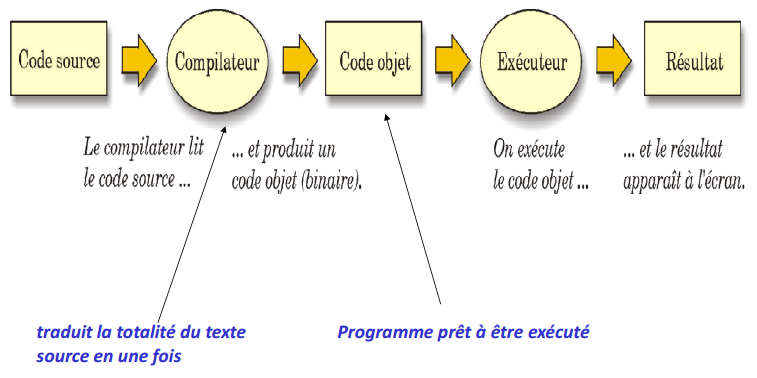
\includegraphics[height=100px, width=400px]{schema.jpg}
        \caption{Schéma bilan sur la transformation du code source}
        \label{Schéma bilan sur la transformation du code source}
    \end{figure}

%----------------------------------------------------------------------------------------

    \newpage

%----------------------------------------------------------------------------------------

    Il convient de noter qu'il est parfois possible de vérifier un programme informatique, c'est-à-dire prouver, de manière plus ou moins automatique, qu'il assure certaines propriétés.\\

%----------------------------------------------------------------------------------------

    \section{Techniques de programmation}
    On retrouve de nombreuses techniques de programmation par exemple la programmation par objet qui consiste à utiliser des techniques de programmation pour mettre en œuvre une conception basée sur les objets. Celle-ci peut être élaborée en utilisant des méthodologies de développement logiciel objet, la programmation  concurrente qui est un paradigme de programmation tenant compte, dans un  programme, de l'existence de plusieurs piles sémantiques qui peuvent être appelées threads, processus ou tâches. Elles sont matérialisées en machine par une pile d'exécution et un ensemble de données privées, ou encore comme la programmation impérative vu précédement.\\

%----------------------------------------------------------------------------------------

    \textbf{Voici une liste de quelques autres techniques de programmation que l'on retrouve dans la programmation informatique}
    \begin{itemize}[leftmargin=50px]
        \item Programmation fonctionnelle
        \item Programmation logique
        \item Programmation orientée prototype
        \item Programmation par contraintes \cite{the}
        \item Programmation structurée
        \label{3}
    \end{itemize}

%----------------------------------------------------------------------------------------

    \newpage  

%----------------------------------------------------------------------------------------

    \bibliographystyle{plain}
    \bibliography{ref.bib}
\end{document}